\documentclass[10pt]{article}
\usepackage[margin=1in]{geometry}
\usepackage{amsmath,amssymb,graphicx,booktabs}
% Standard-font fallbacks for the local TeX installation.
\DeclareFontShape{OT1}{cmr}{m}{n}{<->cmr10}{}
\DeclareFontShape{OT1}{cmr}{bx}{n}{<->cmbx10}{}
\DeclareMathSizes{8}{10}{7}{7}
\DeclareMathSizes{9}{10}{7}{7}
\DeclareMathSizes{10}{10}{7}{7}
\DeclareMathSizes{12}{12}{7}{7}
\ifdefined\XeTeXversion
\DeclareFontShape{TU}{lmr}{m}{n}{<->\UnicodeFontFile{lmroman10-regular}{\UnicodeFontTeXLigatures}}{}
\DeclareFontShape{TU}{lmr}{bx}{n}{<->\UnicodeFontFile{lmroman10-bold}{\UnicodeFontTeXLigatures}}{}
\DeclareFontShape{TU}{lmr}{m}{it}{<->\UnicodeFontFile{lmroman10-italic}{\UnicodeFontTeXLigatures}}{}
\fi
\title{A Detailed Explanation of the Wave Figures}
\author{}
\date{}
\begin{document}
\maketitle

\section{Which figures and which equation?}
This note explains the two drawings in the beginner's guide and the computed moving close-up, space--time map, interference comparison, phase-colored surface, and magnitude level surfaces. The first two drawings are teaching illustrations. The other figures describe a particular computed two-packet solution. Keeping that distinction explicit prevents a convenient sketch from being mistaken for evidence about the equation.

The computed figures use the linear canonical equation
\begin{equation}
 u_t+u_{xxx}-3u_{xyy}-3u_{xzz}=0.
 \label{eq:pde}
\end{equation}
This is the linear model used in the formal checkpoint, not the later nonlinear spatial Dysthe collision experiment. Its initial field is
\begin{equation}
 u(0,x,y,z)=\frac{1}{Z}\left[
 e^{-((x+5)^2+y^2+z^2)/18}
 +0.7i e^{-((x-5)^2+y^2+z^2)/18}\right].
 \label{eq:initial}
\end{equation}
The first packet is centered at $x=-5$, the second at $x=5$. Each Gaussian has width parameter $3$. The second has relative coefficient $0.7$ and a quarter-cycle phase offset, represented by multiplication by $i$. The fixed divisor is approximately $Z=695.2418714$, chosen from the original grid's initial $L^1$ normalization. It is not recomputed as time evolves.

Write
\begin{equation}
 u=Ae^{i\phi},\qquad A=|u|\geq0.
 \label{eq:polar}
\end{equation}
Then $A$ is envelope magnitude and $\phi$ is phase. This representation requires no literal complex-valued water surface: a complex number stores two pieces of wave information together. The analogy is an arrow whose length is $A$ and whose direction is $\phi$.

The coordinates are dimensionless canonical coordinates. These figures are informative about the model's wave-pattern evolution, but they are not calibrated predictions of metres of water elevation, seconds of laboratory time, or fluid-particle velocities. No conversion to such measurements has been supplied here.

\section{The envelope-and-phase illustration}
\begin{figure}[!htbp]
\centering
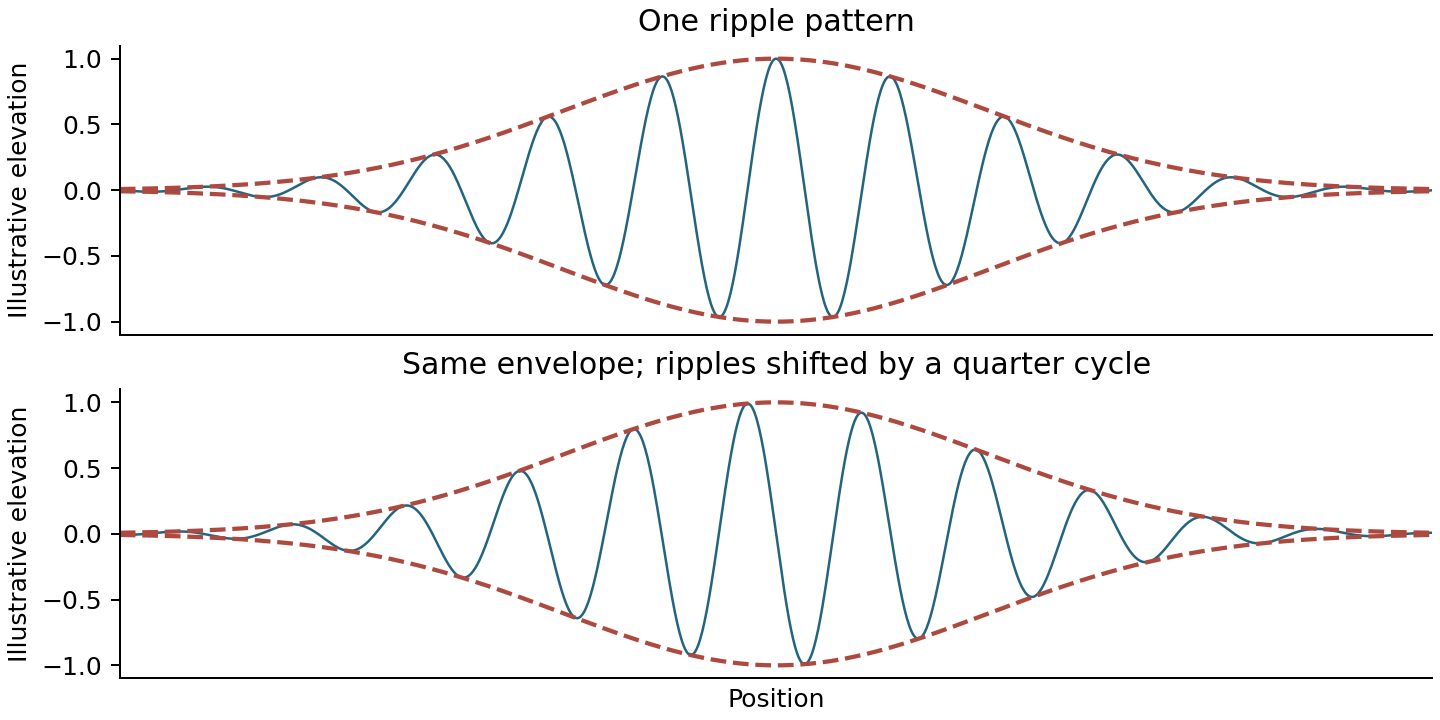
\includegraphics[width=\linewidth]{figures/envelope_and_phase.png}
\caption{Teaching illustration from the beginner's guide. Dashed curves show the same envelope bounds in both panels. Only the phase of the oscillating curve changes. These curves are not saved solutions of equation~\eqref{eq:pde}.}
\label{fig:envelope}
\end{figure}

\subsection{What the curves represent}
In Figure~\ref{fig:envelope}, the dashed outline is $\pm A(x)$ and the oscillating curve has the illustrative form
\begin{equation}
 \eta_{\mathrm{ill}}(x)=A(x)\cos(k_cx+\phi).
 \label{eq:carrier}
\end{equation}
The drawing uses $A(x)=e^{-x^2/30}$ and $k_c=3$. The upper panel uses $\phi=0$ and the lower panel uses $\phi=\pi/2$.

The broad outline answers ``how large can the local oscillation be?'' The rapidly oscillating line answers ``where are the crests and troughs within that outline?'' A positive envelope does not mean the surface is always above its resting level: the cosine still takes both positive and negative values.

In a suitable leading-order water-wave interpretation, $A$ would be related to ripple amplitude after restoring physical units. Here equation~\eqref{eq:carrier} is a drawing convention used to make amplitude and phase visible. The choice $k_c=3$ is illustrative; it was not inferred from measured water data.

\subsection{What changes between the panels}
Adding $\pi/2$ advances the local oscillation by a quarter cycle. Where the first pattern might have a crest, the shifted one may cross its middle level. Both remain within the same dashed bounds. Thus amplitude alone cannot specify the crest positions.

For a constant phase shift, the carrier displacement is $-\Delta\phi/k_c$ in this convention. That is a shift of the oscillatory factor, not necessarily a translation of the entire packet, because the envelope $A(x)$ remains fixed. This distinction is why phase alignment and position alignment are separate operations in the numerical work.

\subsection{What it does not show}
The drawing does not give fluid velocity, pressure, or particle trajectories. Nor does changing its phase prove that one packet moves faster than another. It establishes only the prerequisite idea: equal envelopes can contain different oscillatory patterns.

\section{The height-normalization illustration}
\begin{figure}[!htbp]
\centering
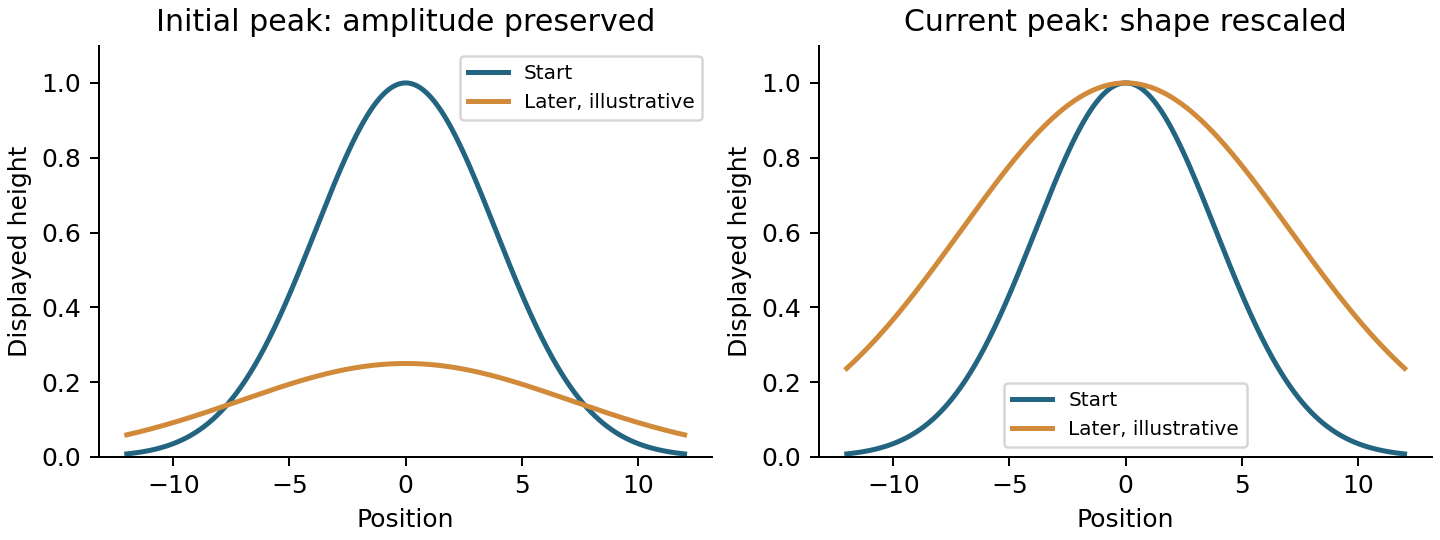
\includegraphics[width=\linewidth]{figures/normalization.png}
\caption{Teaching illustration of the viewer's height settings. The later curve has lower amplitude and greater width. Dividing by each curve's own maximum makes both peaks appear equally tall.}
\label{fig:normalization}
\end{figure}

Let $P_0$ denote the initial reference peak and $P(t)$ the sampled peak in the current viewing region. The two plotted heights are
\begin{equation}
 H_{\mathrm{initial}}=\frac{|u|}{P_0},\qquad
 H_{\mathrm{current}}=\frac{|u|}{P(t)}.
 \label{eq:scales}
\end{equation}
In the illustration, the initial curve is $e^{-x^2/30}$ and the later curve is $0.25e^{-x^2/100}$. The left panel retains the factor $0.25$; the right panel divides it away. These illustrative curves are not asserted to solve the PDE or conserve any integral.

The current-peak setting is useful because otherwise a late solution may look nearly flat. It reveals shoulders, asymmetry, and oscillatory tails. However, it removes the very amplitude decrease that a decay study seeks to measure. The two settings answer different questions: ``what is its shape now?'' and ``how strong is it compared with the start?''

A tall normalized surface at $t=2056$ therefore does not demonstrate persistent physical strength or a soliton. The plot can be tall because its denominator has become very small. To assess strength, inspect the initial-peak setting or the separately printed peak ratio.

\section{The moving close-up}
\begin{figure}[!htbp]
\centering
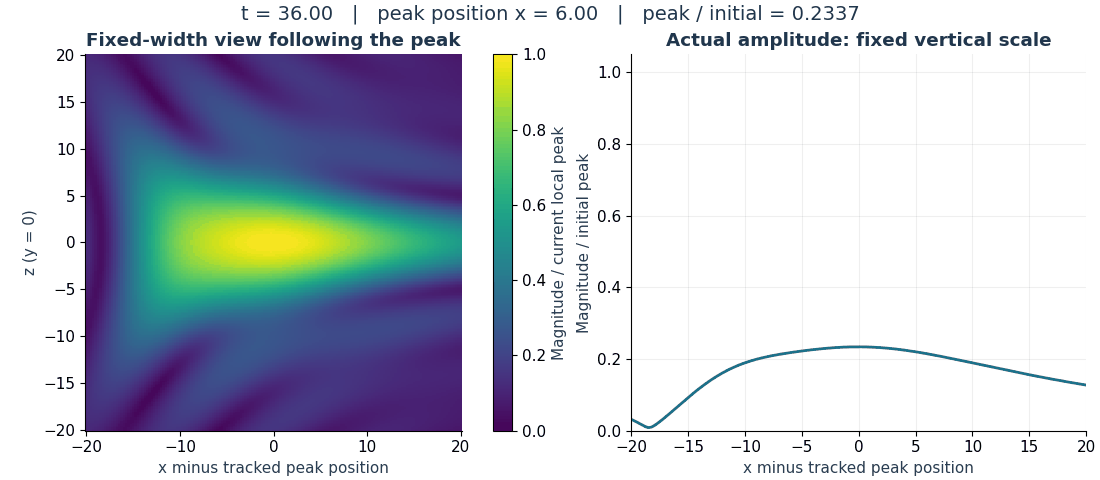
\includegraphics[width=\linewidth]{figures/moving_preview.png}
\caption{One frame of the moving close-up, at $t=36$. The left panel follows the sampled centerline peak with a fixed-width spatial window. The right panel preserves the initial amplitude reference.}
\label{fig:moving}
\end{figure}

\subsection{How the camera follows the packet}
At each saved time the procedure searches the centerline $y=z=0$ over $-24\leq x\leq100$ and selects its largest sampled magnitude. Call the selected position $x_p(t)$. The horizontal coordinate in both panels is
\begin{equation}
 q=x-x_p(t).
\end{equation}
Consequently $q=0$ follows the selected peak even when its position in the original coordinate system changes. The window remains $-20\leq q\leq20$. This avoids the visual problem of the core shrinking to a few pixels when a much wider view is used to retain the outer ripples.

The peak locations measured in this sequence include $x_p(0)=-5$, $x_p(8)=-3$, $x_p(64)=8.25$, and $x_p(256)=17$. These are sampled feature positions, not fluid-particle positions or measurements of a universal propagation speed. If two peaks exchange which is taller, a maximum-following camera can switch between them. It does not assign a permanent identity to a crest.

\subsection{Reading the two panels together}
The left panel uses current local peak normalization, so a bright central region can remain visible throughout the animation. Changes in its width, asymmetry, and surrounding ripples describe shape within this moving window. Some features may enter or leave the window; their disappearance there does not mean they have ceased to exist.

The right panel divides the centerline magnitude by $P_0$ and fixes the vertical range. It therefore shows the local loss of amplitude directly. At $t=36$, the two panels are consistent: the left displays a prominent normalized structure while the printed peak ratio is only about $0.234$.

The animation contains 73 computed times through $256$. Its sampling is finer early and coarser late, so playback is not a uniform clock across the entire movie. The printed time must be used when comparing rates of change.

\section{The space--time diagram}
\begin{figure}[!htbp]
\centering
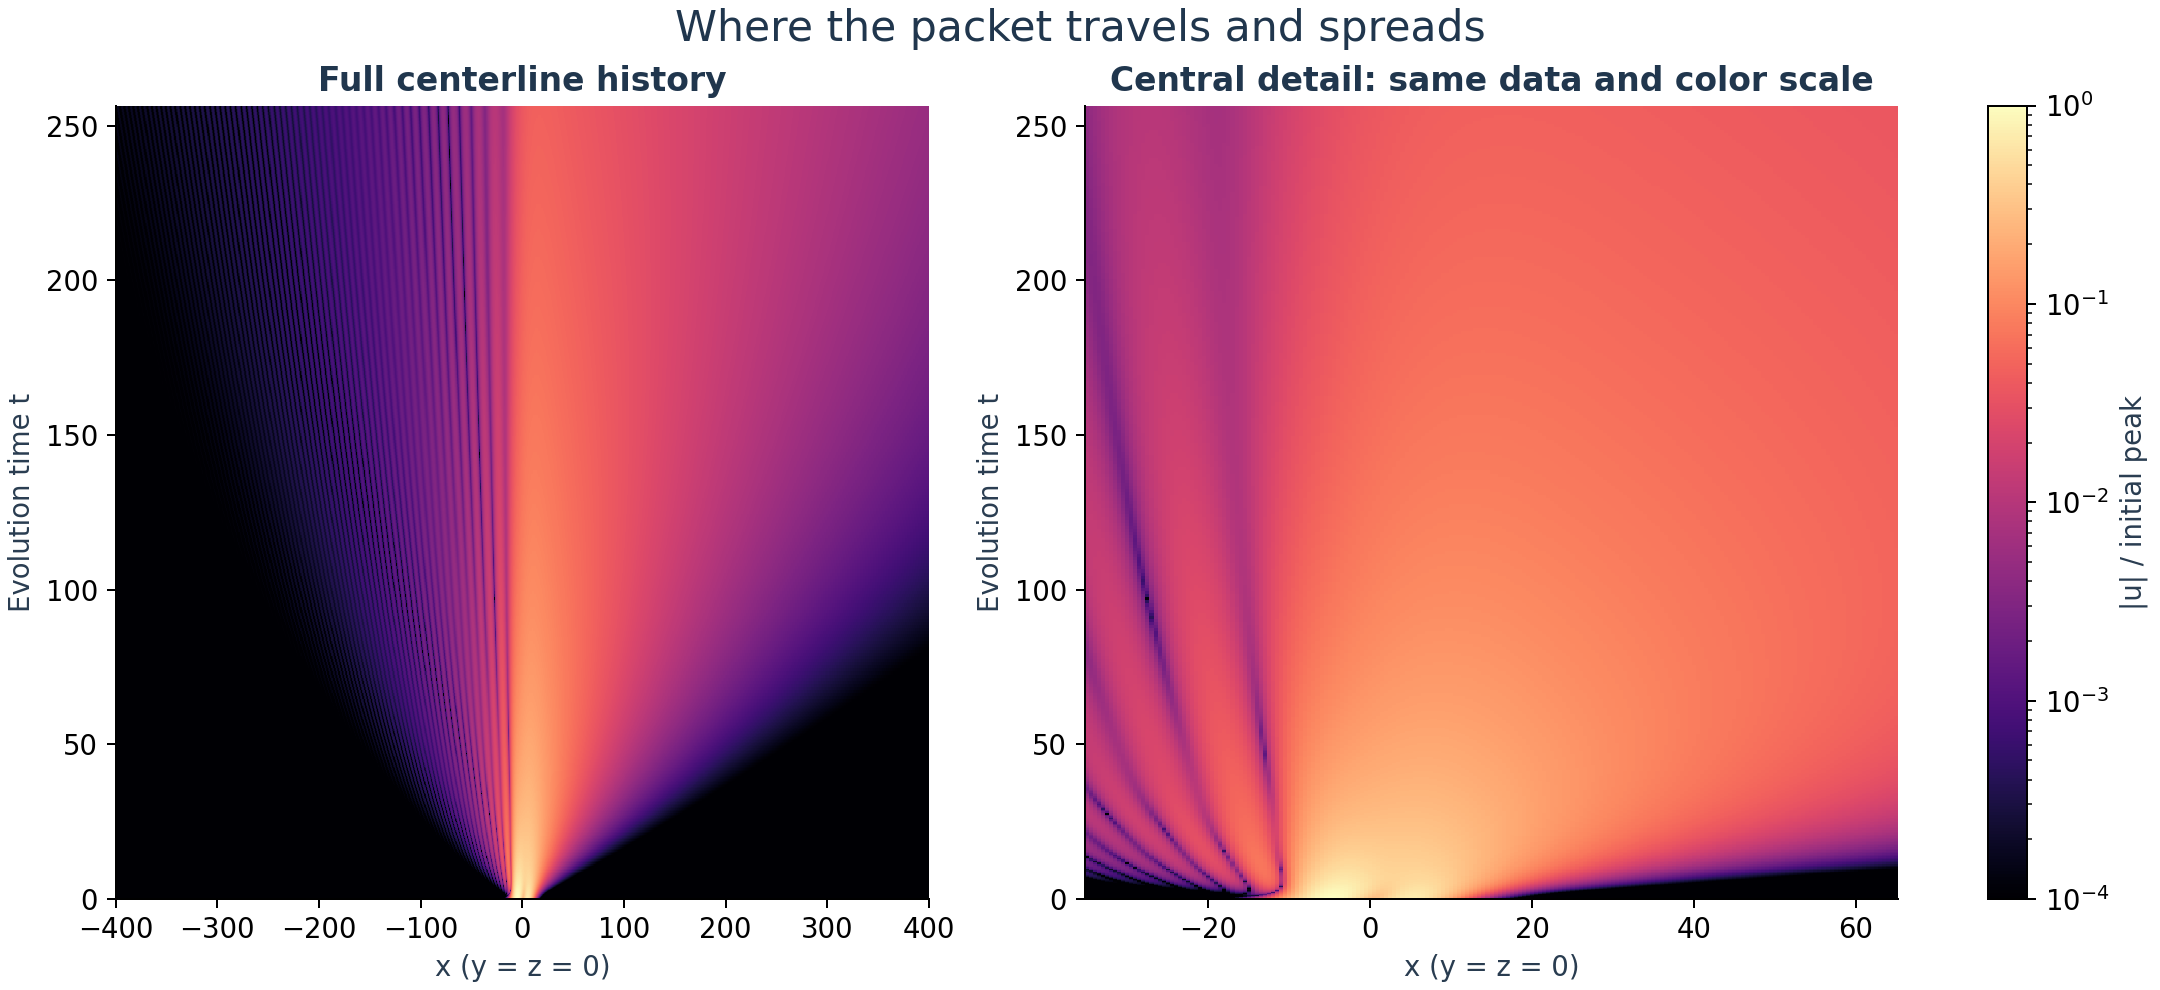
\includegraphics[width=\linewidth]{figures/space_time.png}
\caption{Centerline magnitude as a function of position and evolution time. Both panels use the same logarithmic color scale, normalized by the initial reference peak. The right panel enlarges the central region of the left panel.}
\label{fig:spacetime}
\end{figure}

\subsection{Each row is one snapshot}
In Figure~\ref{fig:spacetime}, position runs horizontally and evolution time runs vertically. Color shows the centerline magnitude divided by the initial reference peak. Reading horizontally is like taking a centerline slice at a fixed time. Reading vertically at one $x$ shows how the amplitude at that fixed position changes.

There are 369 computed time rows from $0$ to $256$. They are placed at their actual time coordinates, even though the numerical sampling intervals differ. This distinguishes the diagram from a movie played with equal duration per frame.

\subsection{What the streaks and spreading region mean}
A sloping band indicates that a magnitude feature changes position. A band whose position satisfies $x\approx vt$ would have the corresponding constant pattern velocity $v$, but a visible band need not follow a straight line or represent one enduring object. A widening colored region indicates that appreciable amplitude is found over a larger range of positions.

The repeated light and dark bands toward negative $x$ are oscillatory structure in the evolved envelope magnitude. They are not automatically the fast physical carrier crests. No extra carrier was multiplied into this plot.

The broad view reveals distant structure that would be missed in the close-up. The central panel makes the strongest region and nearby minima easier to distinguish. Neither panel is a whole-space view: the broad horizontal range is limited to $[-400,400]$, and the data are only the centerline. An off-axis maximum could be missed by any centerline-only plot.

\subsection{Why the color scale is logarithmic}
The scale runs from $10^{-4}$ to $1$. Equal changes along the legend correspond to multiplication of amplitude, not equal additions. A feature at $10^{-3}$ is one thousandth of the initial reference peak, even if its color is easy to see. The logarithmic scale reveals weak ripples without suggesting that they are comparable in amplitude to the core. Values below the color floor cannot be visually distinguished from one another.

\section{The interference comparison and its correction}
\begin{figure}[!htbp]
\centering
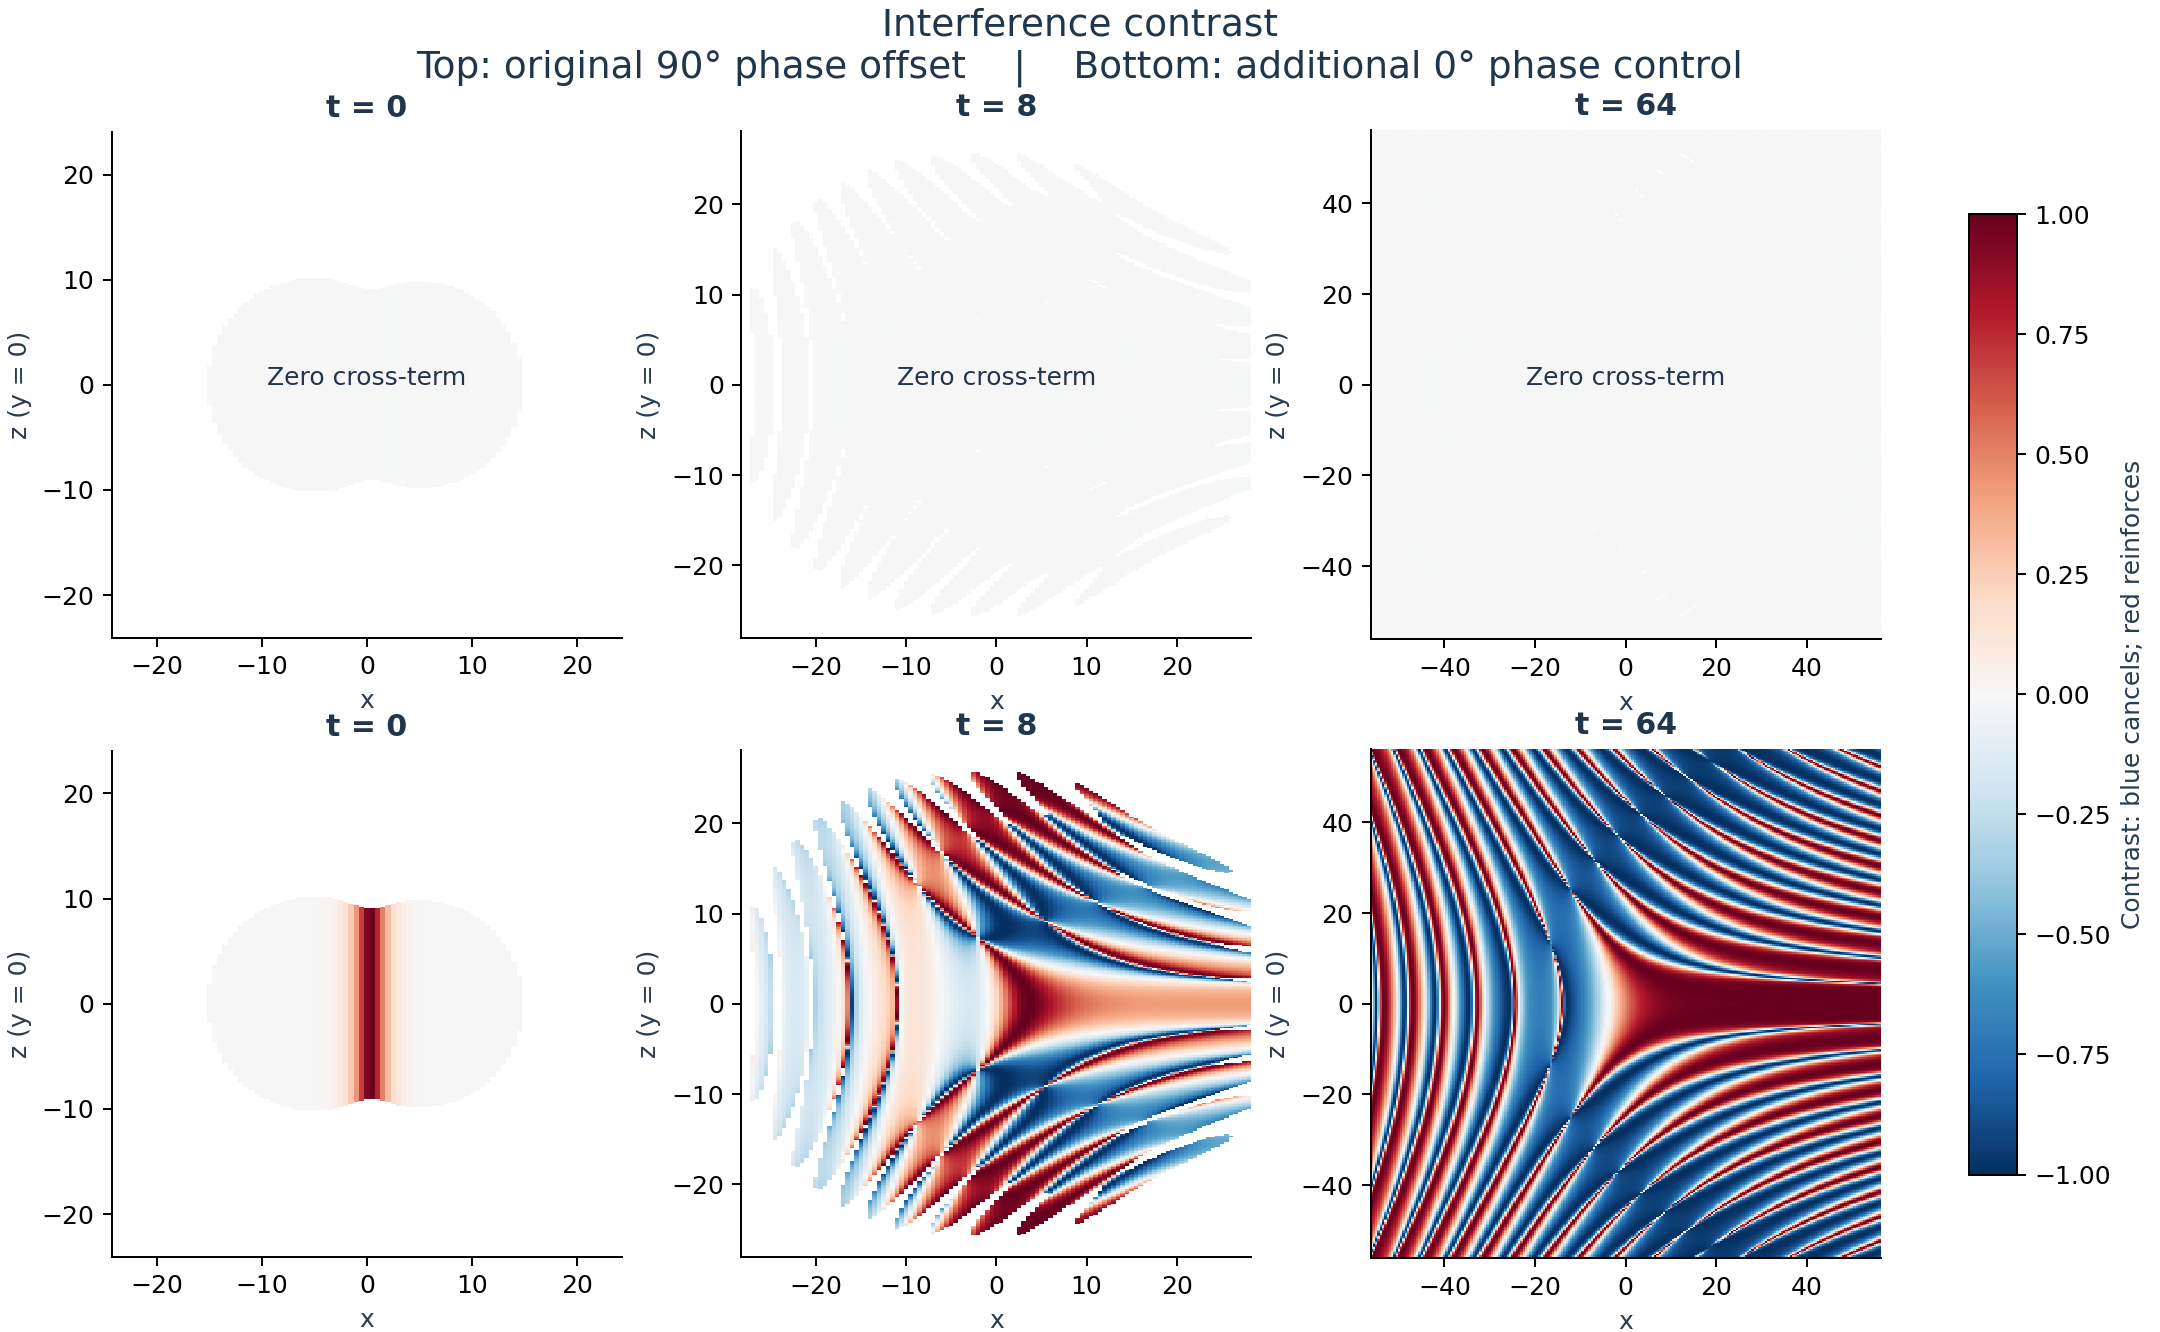
\includegraphics[width=\linewidth]{figures/interference_control.png}
\caption{Interference contrast for the original quadrature pair (top) and an additional zero-phase-offset control (bottom). Red is positive cross-term and blue is negative cross-term. White regions with text indicate the original pair's zero cross-term; weak component-intensity regions are masked.}
\label{fig:interference}
\end{figure}

\subsection{The quantity being isolated}
For two contributions $u_1,u_2$,
\begin{equation}
 |u_1+u_2|^2=|u_1|^2+|u_2|^2+
        2\operatorname{Re}(u_1\overline{u_2}).
 \label{eq:cross}
\end{equation}
The last term is the extra squared amplitude associated with their relative phase. A positive term means reinforcement relative to the sum of separate squared amplitudes. A negative term means cancellation relative to that sum. This is a precise meaning of interference; it is not simply the fact that two visible regions overlap.

To show the sign and relative importance of that term, the plot uses
\begin{equation}
 C_{\mathrm{int}}=
 \frac{2\operatorname{Re}(u_1\overline{u_2})}
 {|u_1|^2+|u_2|^2},\qquad -1\leq C_{\mathrm{int}}\leq1.
 \label{eq:contrast}
\end{equation}
The bound follows from $2|u_1||u_2|\leq|u_1|^2+|u_2|^2$. A contrast near $1$ indicates strong relative reinforcement; a value near $-1$ indicates strong relative cancellation. Either can occur in a weak-amplitude region, so contrast is not a substitute for an absolute magnitude plot.

Regions where the component-sum intensity is below $10^{-5}$ of its spatial peak in that panel are masked. This avoids dividing by negligible numbers and displaying strong-looking contrast where the field is practically absent.

\subsection{Why the top row is zero}
Equation~\eqref{eq:pde} has real coefficients and preserves real initial data. Let $a(t,X)$ and $b(t,X)$ be the real evolved Gaussian profiles, including the common normalization. Then the original initial phase choice gives
\begin{equation}
 u(t,X)=a(t,X)+0.7i\,b(t,X),
\end{equation}
so
\begin{equation}
 |u|^2=a^2+0.49b^2,
 \qquad 2\operatorname{Re}\{a\overline{0.7i b}\}=0.
 \label{eq:zero}
\end{equation}
This is an identity at all times, not just a numerical observation at $t=0$. The computed unmasked contrast is below approximately $1.6\times10^{-14}$ in these panels, consistent with roundoff.

The earlier description of this original pair as developing a nonzero intensity cross-term was incorrect. Its component intensities spread and overlap, changing the total outline, while remaining in quadrature. Individual real components can develop their own oscillatory structure; that does not require mutual intensity interference between the quadrature pair.

\subsection{What is different in the bottom row}
The control changes only the initial phase coefficient from $0.7i$ to $0.7$, keeping the common divisor $Z$. Thus $u=a+0.7b$, and the cross-term becomes $1.4ab$. Initially both Gaussian profiles are positive and the overlap reinforces. Later the real evolved components can change sign in different places, producing alternating regions of reinforcement and cancellation.

This is a deliberately different initial condition, not a different rendering of the original field. It is not independently renormalized to initial $L^1=1$. Its contrast is useful because the common overall amplitude scale cancels in equation~\eqref{eq:contrast}. The red and blue colors here must not be confused with the cyclic colors in the phase view.

\section{The phase-colored envelope surface}
\begin{figure}[!htbp]
\centering
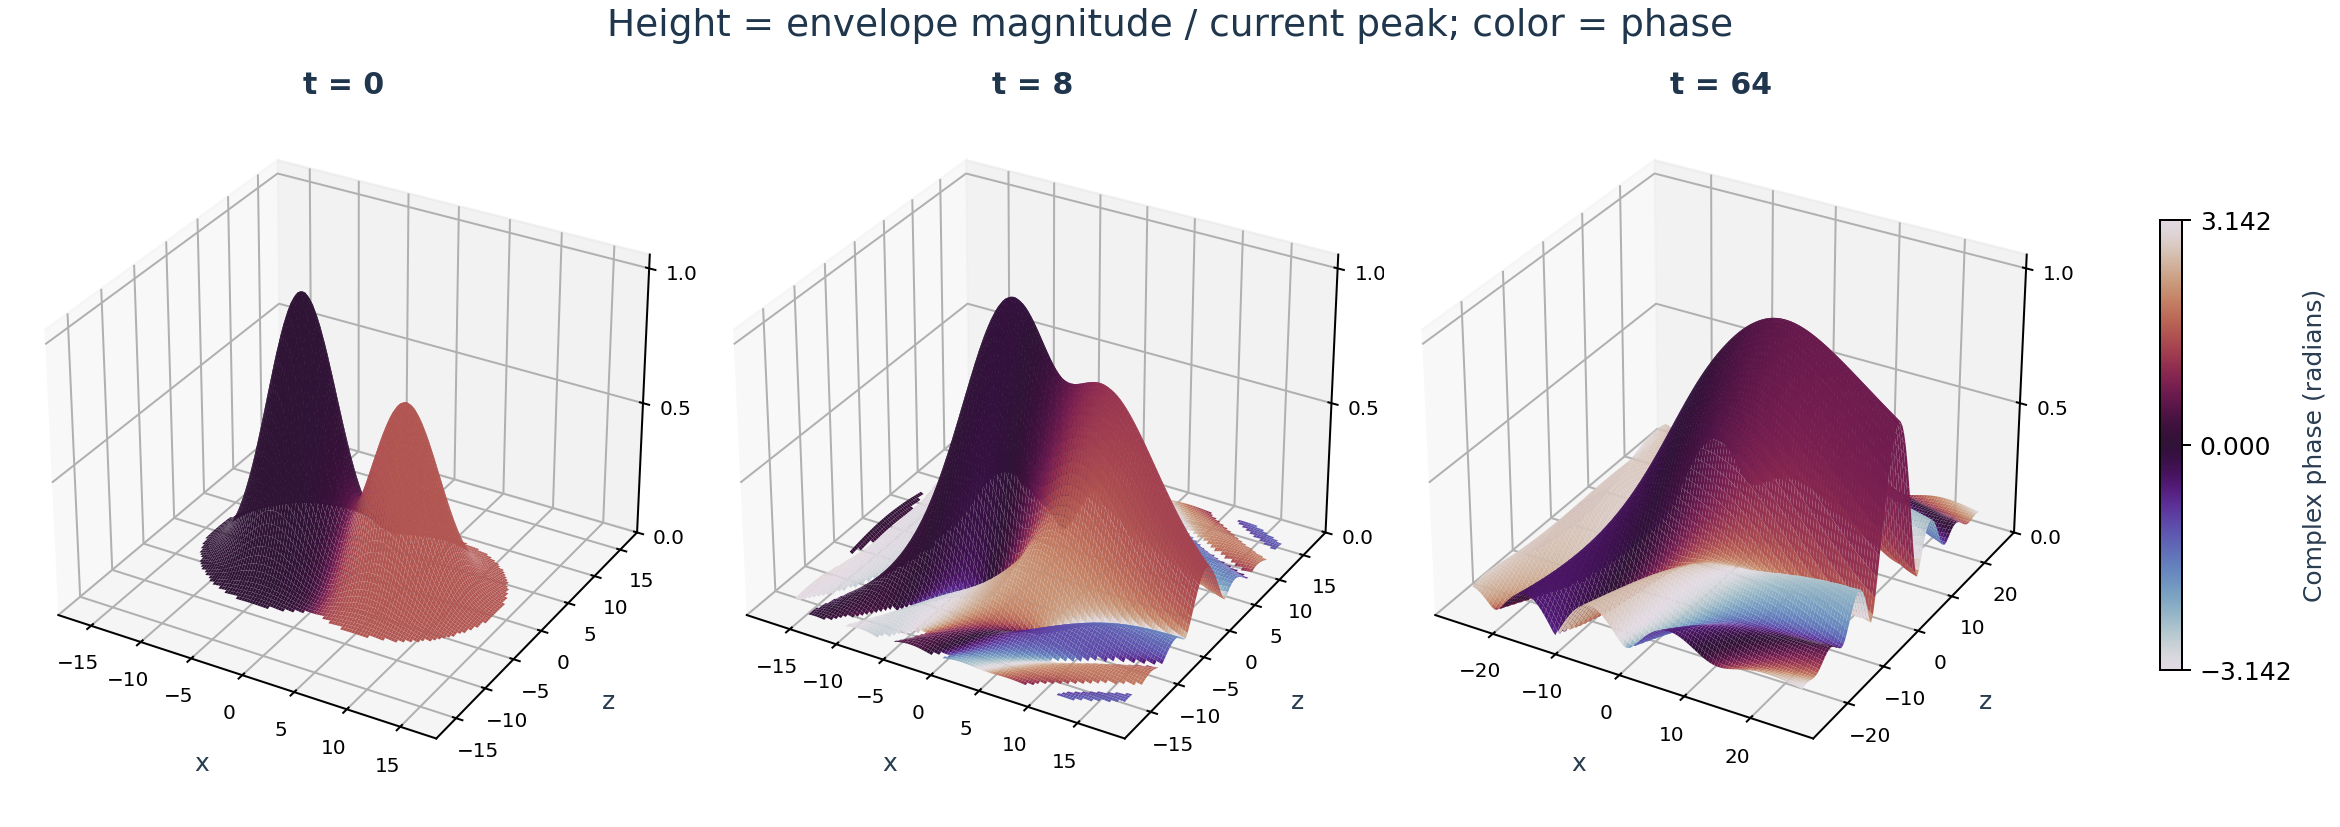
\includegraphics[width=\linewidth]{figures/phase_surface.png}
\caption{Phase-colored magnitude surfaces at $t=0,8,64$. Horizontal coordinates are $x,z$ with $y=0$; height is magnitude divided by the current view peak. Color represents the argument of the combined complex field. Spatial viewing ranges vary between panels.}
\label{fig:phase}
\end{figure}

\subsection{Height and color describe different properties}
Figure~\ref{fig:phase} combines the two pieces of information in equation~\eqref{eq:polar}. Height answers how strong the envelope is relative to the selected amplitude reference. Color answers which phase the combined field has at that location. A ridge of equal height can contain several phases; a region of similar phase can have strongly varying height.

For the original pair, the combined phase can be written schematically as
\begin{equation}
 \phi=\operatorname{atan2}(0.7b,a).
\end{equation}
As the relative sizes and signs of $a$ and $b$ vary, this angle varies. Therefore a rich phase picture is perfectly compatible with the zero intensity cross-term in equation~\eqref{eq:zero}. ``The phase varies'' and ``the two contributions have a nonzero intensity cross-term'' are different claims.

\subsection{Reading color transitions}
The phase is defined modulo $2\pi$. The values $-\pi$ and $\pi$ represent the same direction, so a cyclic palette joins those ends. A sudden-looking numerical wrap in the argument need not be a physical discontinuity. Read phase colors using the current legend: the static figures and the theme-aware interactive viewer need not use identical hues.

Fine bands in color reveal spatial phase variation. They do not indicate temperature bands, pressure fronts, or rotating fluid. Near a zero of the combined field, the phase becomes poorly defined; the viewer omits sufficiently small magnitudes rather than presenting those colors as robust physical structure.

\subsection{The interactive version through $t=2056$}
The extended viewer contains 122 computed snapshots. Its time intervals are $1$ through $t=16$, $2$ through $64$, $8$ through $256$, and $32$ through $2048$, followed by a final sample at $2056$. The transition intervals are read from the actual listed times. The slider indexes these snapshots; it does not create a continuously computed solution between them.

The rotation and tilt controls change the camera only. The current-peak height setting emphasizes geometry; the initial-peak setting retains amplitude decay. The central viewing halfwidth follows $16+0.15t$ through $256$ and then grows proportionally to $(t/256)^{1/3}$, reaching about $109$ at $2056$. This is a display choice to keep the core readable, not a measured spreading law or a proof of self-similarity.

The displayed mesh has $65\times65$ samples. For compact interactive storage, magnitude and phase are quantized to 8 bits each after the complex double-precision calculation. This limits display precision; it does not change the precision of the underlying field calculation. Subtle color or surface facets should not be interpreted below that display resolution.

\section{Magnitude level surfaces: a different kind of 3D view}
\begin{figure}[!htbp]
\centering
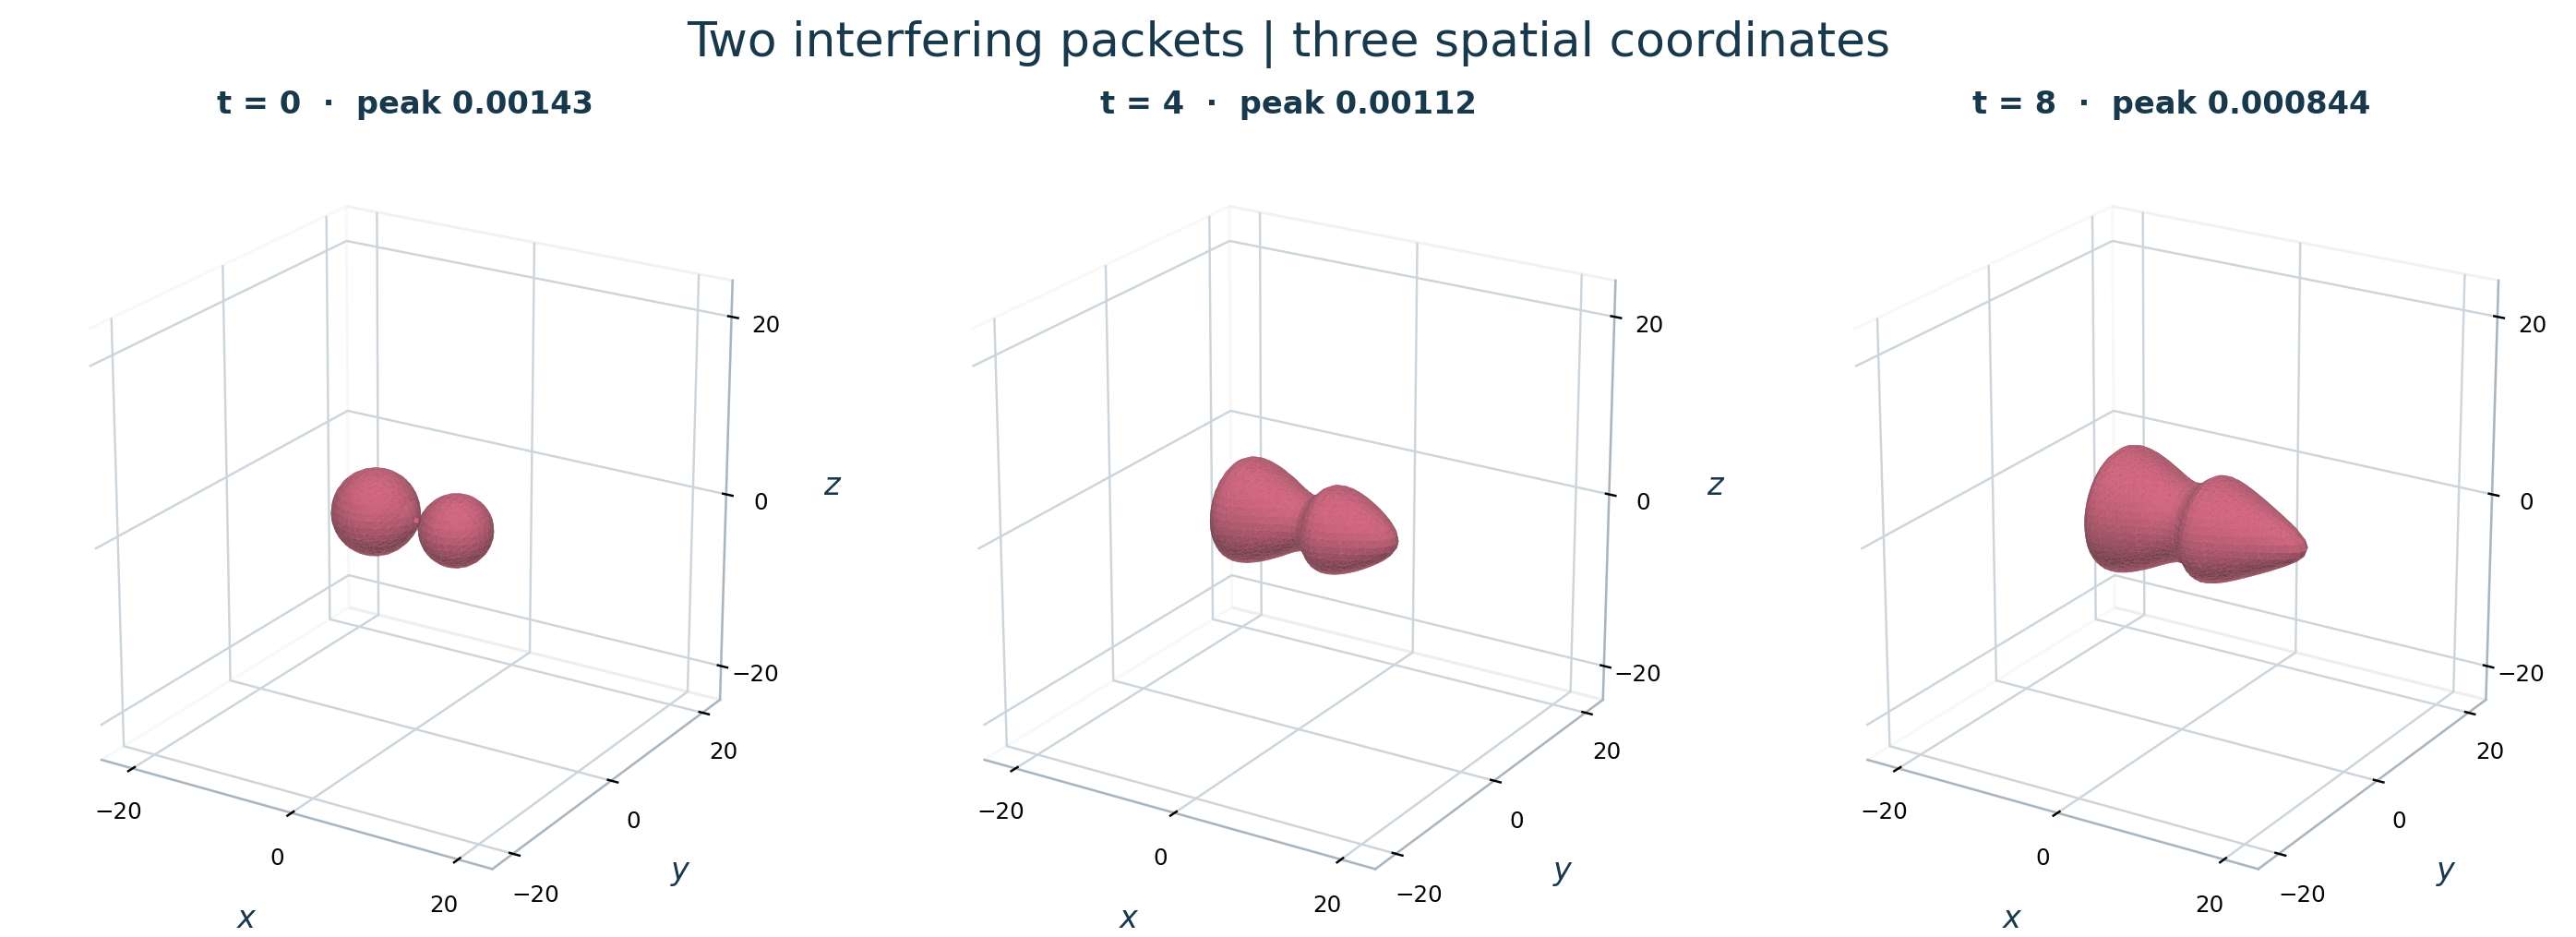
\includegraphics[width=\linewidth]{figures/level_surfaces.png}
\caption{Earlier magnitude level-surface views of the same quadrature pair, at $t=0,4,8$. Each surface uses 30\% of that snapshot's peak. The historical title ``interfering packets'' should be read with the correction in Section~6: the original pair has no mutual intensity cross-term.}
\label{fig:levels}
\end{figure}

The phase-colored surface is a height graph above a two-coordinate slice. In contrast, a magnitude level surface is the set of points in all three coordinates satisfying
\begin{equation}
 \Sigma_\theta(t)=\{(x,y,z):|u(t,x,y,z)|=\theta P(t)\}.
\end{equation}
Here $x,y,z$ are all spatial coordinates of the model. No axis is used to display amplitude as a height. The surface is comparable to a three-dimensional contour line: it locates a chosen magnitude value in space.

The interactive level-surface viewer offers $\theta=0.1,0.3,0.6$ at $t=0,8,64,256$. A high threshold emphasizes the core; a lower threshold reveals more extended structures. Distinct connected pieces can appear or join when either the field or the threshold changes. Such a change is not automatically a physical merger of material objects.

For this input and equation, the field is radially symmetric in the transverse coordinates $y,z$. The interactive geometry is constructed by computing contours in $(x,r)$, where $r=\sqrt{y^2+z^2}$, and revolving them about the $x$ axis. This uses the actual symmetry of the numerical solution rather than an arbitrary assumed shape.

The reference $P(t)$ and the camera fit change between snapshots. A surface occupying much of the screen at late time may represent a much smaller absolute amplitude. To compare a fixed physical threshold, one would need to hold the threshold in absolute units instead; that is not what the current percentage controls do.

\section{What the figures say about physical spreading and decay}
\subsection{Local weakening is not necessarily dissipation}
For the Fourier convention used here,
\begin{equation}
 \widehat u(t,k)=e^{itw(k)}\widehat u(0,k),\qquad
 w(k)=k_x^3-3k_x(k_y^2+k_z^2).
\end{equation}
Since $|e^{itw}|=1$, the linear evolution changes phases in Fourier space but preserves Fourier magnitudes. For sufficiently localized solutions, this implies conservation of the whole-space squared norm:
\begin{equation}
 \int |u(t,X)|^2\,dX=\int |u(0,X)|^2\,dX.
\end{equation}
The peak may nevertheless decrease because the pattern is distributed differently across space. Thus local weakening and conservation of an integrated quantity can occur together. The equation contains no damping term. Calling this conserved quantity a measured fluid energy would require a physical model and normalization beyond the present visualization.

\subsection{The measured peak ratios}
The extended phase viewer reports the following sampled central-view values:
\begin{center}
\begin{tabular}{rrr}
\toprule
$t$ & $P(t)/P_0$ & Percentage of initial reference peak\\
\midrule
0 & 1.000000 & 100.0000\\
8 & 0.586365 & 58.6365\\
64 & 0.153352 & 15.3352\\
256 & 0.0465254 & 4.65254\\
512 & 0.0244108 & 2.44108\\
1024 & 0.0126006 & 1.26006\\
2056 & 0.00641199 & 0.641199\\
\bottomrule
\end{tabular}
\end{center}
Different plots use different display meshes, so their sampled peaks can differ slightly. This table identifies the extended phase-view data rather than mixing values from separate grids.

The squared peak ratio at the final listed time is approximately $4.11\times10^{-5}$. That is a comparison of peak squared magnitudes, not a statement that only that fraction of the total signal remains. The integral above is a different quantity and can remain constant.

These figures plot the unweighted envelope. The earlier $t^{-7/6}$ question concerns a specified weighted linear observable and its norms. Rescaled pictures, a few unweighted peak ratios, or a fitted slope for one input cannot strengthen or refute that uniform statement on their own.

\subsection{Numerical reliability and physical reliability}
The late-time field was not obtained by merely stretching an early image. The transverse Gaussian integrals are evaluated analytically, while a longitudinal Fourier quadrature is enlarged with time. At $t=2056$, the longitudinal period is $65536$ with $262144$ quadrature nodes.

At selected times, the calculation was repeated with twice the period at fixed spacing and half the spacing at fixed period. On identical displayed coordinates, the largest checked spacing-change relative field discrepancy was about $0.0302\%$; at $2056$ it was about $0.00162\%$. These are useful consistency checks on the displayed field, not rigorous whole-space error bounds or validation against a laboratory fluid.

There are therefore three separate questions: whether the numerical integral is accurate, whether the rendering resolves what was computed, and whether the mathematical model represents a particular physical experiment. The reported checks address the first question locally. Mesh size, thresholds, and color scales constrain the second. Physical calibration and comparison with suitable measurements would be needed for the third.

\section{A practical sequence for reading the figures}
Start with the envelope-and-phase illustration to separate outline from crests. Next compare the two normalization settings so that a persistent displayed height is not mistaken for persistent amplitude. Then use the moving close-up for local shape and the space--time diagram for motion and spreading across the full interval.

Use the interference comparison to ask whether overlap creates an extra squared-amplitude term. For the original quadrature pair the answer is no; the added zero-phase control illustrates the alternative. Use the phase-colored surface to inspect the combined field's angle, which remains meaningful as separate information even in the absence of a mutual intensity cross-term.

Finally rotate the magnitude level surfaces to inspect three-coordinate geometry. Check their threshold and camera scale before comparing sizes. Return to the initial-peak setting or the numerical peak ratio whenever the question is decay rather than shape.

\section*{Source of the figures and values}
The teaching drawings are from the beginner's guide. Computed views and component checks are recorded in the packet alternative-view outputs; the original level-surface image is from the formal checkpoint's figure-review collection. The extended phase viewer's metadata and refinement checks provide the long-time values above. All use the specific initial data~\eqref{eq:initial} unless a separate phase-control input is explicitly identified. This note changes no simulation data and retains the correction to the earlier interpretation of the original pair's interference.
\end{document}
